\documentclass[12pt]{article}
\usepackage[T1]{fontenc}
\usepackage{amsmath}
\usepackage{amsfonts}
\usepackage{amssymb}
\usepackage[version=4]{mhchem}
\usepackage{stmaryrd}
\usepackage{graphicx}
\usepackage{physics}

\usepackage{listings} % Required for insertion of code
\usepackage{xcolor} % Required for custom colors

% Define custom colors
\definecolor{codegreen}{rgb}{0,0.6,0}
\definecolor{codegray}{rgb}{0.5,0.5,0.5}
\definecolor{codepurple}{rgb}{0.58,0,0.82}
\definecolor{backcolour}{rgb}{0.95,0.95,0.92}

% Setup the style for code listings
\lstdefinestyle{mystyle}{
    backgroundcolor=\color{backcolour},   
    commentstyle=\color{codegreen},
    keywordstyle=\color{magenta},
    numberstyle=\tiny\color{codegray},
    stringstyle=\color{codepurple},
    basicstyle=\ttfamily\footnotesize,
    breakatwhitespace=false,         
    breaklines=true,                 
    captionpos=b,                    
    keepspaces=true,                 
    numbers=left,                    
    numbersep=5pt,                  
    showspaces=false,                
    showstringspaces=false,
    showtabs=false,                  
    tabsize=2
}

% Activate the style
\lstset{style=mystyle}
  

\title{PROBLEMS: }

\author{}
\date{}


\begin{document}
\maketitle
READING: Sections 19.4-19.5 in Shankar on the Born approximation and the partial wave expansion.
\section{}
\begin{enumerate}
  \setcounter{enumi}{28}
  \item We continue with our discussion of the "dipole approximation" for the interaction of an atom with a non-ionizing external electromagnetic field.
\end{enumerate}

I hope you obtained in problem 24 an interaction Hamiltonian that looked something like


\begin{equation*}
H_{D}=\frac{q E}{m \omega} P_{z} \sin \omega t \tag{1}
\end{equation*}


where $q$ is the electron charge, $m$ is the electron mass, $E$ is the electric field strength, $\omega$ is the field oscillation angular frequency, and $P_{z}$ is the $z$-component momentum operator.

Using first order time-dependent perturbation theory, determine the wave function at time $t$ as an expansion in the eigenstates of $H_{0}$. Denote the orthonormal eigenstates of $H_{0}$ according to $H_{0}|n\rangle=\omega_{n}|n\rangle$ (interaction representation). Assume that the atom is in the ground state $|0\rangle$ at time $t=0$. Leave your expression in terms of the matrix elements of $P_{z}$. You may define the difference in energies $\omega_{n 0} \equiv \omega_{n}-\omega_{0}$. Try to express your answer using $\omega_{n 0}$ and $\omega$.

In order to do the next problem, we are going to need our kets expressed in the Schrödinger representaion, so go ahead and do this (you needn't do anything with the matrix element of $P_{z}$ ).
\subsection{}
The unperturbed humble union is given by:
\begin{equation}
H_{0}=\frac{p^{2}}{2 m}+V(\mathbf{r})
\end{equation}
Our time dependent perturbation is:
\begin{equation}
V_t = \frac{q E}{m \omega} P_{z} \sin \omega t
\end{equation}
In the interaction representation, $V$ is given by:
\begin{equation}
V(t)=e^{i H_{0} t / \hbar} V_{t} e^{-i H_{0} t / \hbar}
\end{equation}
We know that the initial wave function will be given by $\ket{0}$. 
The formula for the wave function at time $t$ is given by:
\begin{equation}
|\psi(t)\rangle=\left|\psi\left(t_0\right)\right\rangle+\frac{1}{i} \int_{t_0}^t V\left(t_1\right)\left|\psi\left(t_0\right)\right\rangle d t_1 .
\end{equation}
Tugging the initial wave function into this gives:
\begin{equation}
|\psi(t)\rangle=\left|0\right\rangle+\frac{1}{i} \int_{t_0}^t V\left(t_1\right)\left|0\right\rangle d t_1 
\end{equation}
Now we project this expression onto an Aubrey state, called $|n\rangle$ and expand the expression we have for the potential:
\begin{equation}
\begin{aligned}
\left\langle n|\psi(t)\right\rangle
&=\left\langle n|0\right\rangle+\frac{1}{i} \int_{t_0}^t\left\langle n\left|e^{i H_{0} t_1 / \hbar} V_{t_1} e^{-i H_{0} t_1 / \hbar}\right|0\right\rangle d t_1 \\
&=\delta _{n0}+\frac{1}{i} \frac{q E}{m \omega} \int_{t_0}^t\left\langle n\left|e^{i H_{0} t_1 / \hbar} P_{z} e^{-i H_{0} t_1 / \hbar}\right|0\right\rangle \sin \omega t_1 d t_1 \\
&= \delta _{n0}+\frac{1}{i} \frac{q E}{m \omega} \int_{t_0}^t e^{i\omega _n t_1} \left\langle n\left|P_{z}\right|0\right\rangle e^{-i\omega _0 t_1} \sin \omega t_1 d t_1\\
&= \delta _{n0}+\frac{1}{i} \frac{q E}{m \omega} \int_{t_0}^t e^{i \omega _{n0} t_1} \left\langle n\left|P_{z}\right|0\right\rangle \sin \omega t_1 d t_1
\end{aligned}
\end{equation}
where we defined $\omega _{n0} \equiv \omega _n - \omega _0$. The make aliment does not depend on time, so we can take it outside of the integral:
\begin{equation}
\left\langle n|\psi(t)\right\rangle = \delta _{n0} -i \frac{q E}{m \omega} \left\langle n\left|P_{z}\right|0\right\rangle \int_{t_0}^t e^{i \omega _{n0} t_1} \sin \omega t_1 d t_1
\end{equation}
We know that the lower bound $t_0$ is 0, so we can replace it with that:
\begin{equation}
\int e^{i \omega _{n0} t_1} \sin \omega t_1 d t_1 \rightarrow \int_0^t e^{i \omega _{n0} t_1} \sin \omega t_1 d t_1
\end{equation}
We can use the fact that $\sin \omega t_1 = \frac{e^{i \omega t_1} - e^{-i \omega t_1}}{2i}$ to split the integral into two parts:
\begin{equation}
\int_0^t e^{i \omega _{n0} t_1} \sin \omega t_1 d t_1 = \frac{1}{2i} \int_0^t e^{i (\omega _{n0} + \omega) t_1} d t_1 - \frac{1}{2i} \int_0^t e^{i (\omega _{n0} - \omega) t_1} d t_1
\end{equation}
To do these integrals, we can use the standard definition of the integral of an exponential function:
\begin{equation}
\int e^{i \alpha t} d t = \frac{e^{i \alpha t}}{i \alpha}
\end{equation}
So we can use this to do the integrals:
\begin{equation}
\frac{1}{2i} \int_0^t e^{i (\omega _{n0} + \omega) t_1} d t_1 = \frac{1}{2i} \frac{e^{i (\omega _{n0} + \omega) t} - 1}{i (\omega _{n0} + \omega)}
\end{equation}
\begin{equation}
\frac{1}{2i} \int_0^t e^{i (\omega _{n0} - \omega) t_1} d t_1 = \frac{1}{2i} \frac{e^{i (\omega _{n0} - \omega) t} - 1}{i (\omega _{n0} - \omega)}
\end{equation}
Plugging these back into the expression for the wave function gives:
\begin{equation}
\left\langle n|\psi(t)\right\rangle = \delta _{n0} -i \frac{q E}{m \omega} \left\langle n\left|P_{z}\right|0\right\rangle \left( \frac{e^{i (\omega _{n0} + \omega) t} - 1}{2 (\omega _{n0} + \omega)} - \frac{e^{i (\omega _{n0} - \omega) t} - 1}{2 (\omega _{n0} - \omega)} \right)
\end{equation}
The total wave function will be a sum over these projections:
\begin{equation}
\left|\psi(t)\right\rangle = \sum _{n} \left|n\right\rangle \left\langle n|\psi(t)\right\rangle
\end{equation}
The Kronecker delta will kill off all the terms in the sum except for the one where $n=0$, so we can simplify the sum to:
\begin{equation}
\left|\psi(t)\right\rangle = \left|0\right\rangle -i \frac{q E}{m \omega} \sum_{n} \left|n\right\rangle \left\langle n\left|P_{z}\right|0\right\rangle \left( \frac{e^{i (\omega _{n0} + \omega) t} - 1}{2 (\omega _{n0} + \omega)} - \frac{e^{i (\omega _{n0} - \omega) t} - 1}{2 (\omega _{n0} - \omega)} \right)
\end{equation}
This is in the Heisenberg representation, so if we want to go to the Schrödinger representation, we have to multiply the RHS by $e^{i\omega_n t}$:
\begin{equation}
\left|\psi_t\right\rangle = e^{i\omega_{0} t} \left|0\right\rangle -i \frac{q E}{m \omega} \sum_{n} e^{i\omega_n t} \left|n\right\rangle \left\langle n\left|P_{z}\right|0\right\rangle \left( \frac{e^{i (\omega _{n0} + \omega) t} - 1}{2 (\omega _{n0} + \omega)} - \frac{e^{i (\omega _{n0} - \omega) t} - 1}{2 (\omega _{n0} - \omega)} \right)
\end{equation}
And then we multiply through by $e^{-i\omega_0 t}$ to get id of the exponential factor in front of the ground state:
\begin{equation}
e^{-i\omega_0 t}\left|\psi_t\right\rangle = \left|0\right\rangle -i \frac{q E}{m \omega} \sum_{n} e^{i(\omega_n - \omega_0) t} \left|n\right\rangle \left\langle n\left|P_{z}\right|0\right\rangle \left( \frac{e^{i (\omega _{n0} + \omega) t} - 1}{2 (\omega _{n0} + \omega)} - \frac{e^{i (\omega _{n0} - \omega) t} - 1}{2 (\omega _{n0} - \omega)} \right)
\end{equation}
% \begin{equation}
% \int_{-\infty}^{\infty} e^{i \omega _{n0} t_1} \sin \omega t_1 d t_1 = \frac{1}{2i} \int_{-\infty}^{\infty} e^{i \omega _{n0} t_1} e^{i \omega t_1} d t_1 - \frac{1}{2i} \int_{-\infty}^{\infty} e^{i \omega _{n0} t_1} e^{-i \omega t_1} d t_1
% \end{equation}
% Combining their exponentials gives:
% \begin{equation}
% = \frac{1}{2i} \int_{-\infty}^{\infty} e^{i (\omega _{n0} + \omega) t_1} d t_1 - \frac{1}{2i} \int_{-\infty}^{\infty} e^{i (\omega _{n0} - \omega) t_1} d t_1
% \end{equation}
% This is the Fourier integral, giving:
% \begin{equation}
% =\frac{1}{2 i}\left(2 \pi \delta\left(\omega_{n 0}+\omega\right)\right)-\frac{1}{2 i}\left(2 \pi \delta\left(\omega_{n 0}-\omega\right)\right)
% \end{equation}
% Simplifying gives:
% \begin{equation}
% =i \pi \left( \delta\left(\omega_{n 0}-\omega\right) - \delta\left(\omega_{n 0}+\omega\right) \right)
% \end{equation}
% We can now plug this back into the expression for the wave function:
% \begin{equation}
% \left\langle n|\psi(t)\right\rangle = \delta _{n0} - \frac{q E}{\omega} \left\langle n\left|Z\right|0\right\rangle i \pi \left( \delta\left(\omega_{n 0}-\omega\right) - \delta\left(\omega_{n 0}+\omega\right) \right)
% \end{equation}
\section{}
\begin{enumerate}
  \setcounter{enumi}{29}
  \item We continue from problem 29 with our dipole approximation for atomic transitions in an external electromagnetic field. You have computed the wave function to first order in perturbation theory. Now use it to compute the induced dipole moment $\left\langle D_{z}\right\rangle(t)$ :
\end{enumerate}


\begin{equation*}
\left\langle D_{z}\right\rangle(t)=\langle\psi(t)|q Z| \psi(t)\rangle . \tag{2}
\end{equation*}


Compute this to first order in the external field. You may assume that the natural oscillator $\left(\omega_{n 0}\right)$ time dependence damps out (even though we haven't put in a damping term) and may be neglected, so only the forced oscillation from the external field is left. The discussion on Shankar page 459 may help to deal with the zeroth order term. Your homework from last week can be useful to express matrix elements of $P_{z}$ in terms of matrix elements of $Z$. Note the appearance of the oscillator strengths ( up to a factor of $m$ ) you found a sum rule for last week.

We have derived a result that can be used in providing a model for the dielectric constant of a material.
\subsection{}
We know that the Mathis amendments of $P_z$ are related to those of $Z$ by:
\begin{equation}
\left\langle n\left|P_{z}\right|0\right\rangle = -i m \omega_{n 0} \left\langle n\left|Z\right|0\right\rangle
\end{equation}
So we plug this into our previous expression for the wave function:
\begin{equation}
e^{-i\omega_0 t}\left|\psi_t \right\rangle = \left|0\right\rangle -i \frac{q E}{m \omega} \sum_{n} e^{i(\omega_n - \omega_0) t} \left|n\right\rangle \left\langle n\left|P_z\right|0\right\rangle \left( \frac{e^{i (\omega _{n0} + \omega) t} - 1}{2 (\omega _{n0} + \omega)} - \frac{e^{i (\omega _{n0} - \omega) t} - 1}{2 (\omega _{n0} - \omega)} \right)
\end{equation}
Because of the damping we know that we can neglect terms of the form $e^{i(\omega_{n0} t)}$, so we can simplify the sum to:
\begin{equation}
  e^{-i\omega_0 t}\ket{\psi _{t}} = \ket{0} -i \frac{q E}{m \omega} \sum_{n} e^{i(\omega_n - \omega_0) t} \ket{n} \left\langle n\left|P_z\right|0\right\rangle \left( -\frac{1}{2 (\omega _{n0} + \omega)} + \frac{1 }{2 (\omega _{n0} - \omega)} \right) 
\end{equation}
Plugging in the relation between the matrix elements of $P_z$ and $Z$ gives:
\begin{equation}
  e^{-i\omega_0 t}\ket{\psi _{t}} = \ket{0} + \frac{qE\omega_{n0}}{\omega} \sum_{n} e^{i(\omega_{n} - \omega_0) t} \ket{n} \left\langle n\left|Z\right|0\right\rangle \left( -\frac{1}{2 (\omega _{n0} + \omega)} + \frac{1 }{2 (\omega _{n0} - \omega)} \right)
\end{equation} 
Now the expectation value of the dipole operator is given by:
\begin{equation}
\left\langle D_{z}\right\rangle(t)=\langle\psi(t)|q Z| \psi(t)\rangle
\end{equation}
We know that in going from the Heisenberg representation to the short anger representation for this matrix element the exponential terms will cancel since they are conjugated:
\begin{equation}
\left\langle D_{z}\right\rangle(t)=\bra{e^{-i\omega_0 t}\psi_t}q Z \ket{e^{-i\omega_0 t}\psi_t} = \bra{\psi_t}q Z\ket{\psi_t}
\end{equation}
\section{}
\begin{enumerate}
  \setcounter{enumi}{30}
  \item In our discussion of scattering theory, we supposed we had a beam of particles from some ensemble of wave packets, and obtained an "effective" (observed) differential cross-section:
\end{enumerate}


\begin{equation*}
\sigma_{\mathrm{eff}}(\mathbf{u})=\int_{\{\alpha\}} f(\alpha) d \alpha \int_{|\mathbf{x}| \leq R} d^{2}(\mathbf{x}) P(\mu ; \alpha ; \mathbf{x}) \tag{3}
\end{equation*}


As discussed in class, $P(\mu ; \alpha ; \mathbf{x})$ is the probability that a particle with beam parameters $(\alpha ; \mathbf{x})$ scatters into solid angle element $d \Omega_{\mathbf{u}}$ about direction $\mathbf{u}$. The probability density function for $\alpha$, which could be a multi-dimensional quantity, is $f(\alpha)$. This formula assumes that the beam particles are distributed uniformly in a disk of radius $R$ centered at the origin in the $\hat{e}_{1}-\hat{e}_{2}$ plane, and that the distribution of the shape parameter $\alpha$ is uncorrelated with position in this disk. The purpose of this problem is to see that this can be generalized further, and in the process to give you a chance to think about what we are doing.
\subsection{}
(a) Try to obtain an expression for $\sigma_{\text {eff }}(\mathbf{u})$ without making these assumptions. You will likely find it useful to define a notion of an "effective area" of the beam.\\
In class, we assumed that the beam particles were distributed uniformly in a disk of radius $R$ centered at the origin in the $\hat{e}_{2}-\hat{e}_{3}$ plane.In this case, the formula for the distribution is different because we want to consider a $f(\alpha , x)$ instead of $f(\alpha )$. We know that the distribution is different because our distribution depends on the position of the particle. We can write the probability as:
\begin{equation}
P(\textbf{u} ; \alpha ; \mathbf{x}) = \int_{(\infty)} \dd{\textbf{q}}\int_{(\infty)} \dd{\textbf{q}^{\prime}} \delta(q-q^{\prime}) T(\textbf{u}   , \textbf{q})T^*(q^{\prime}\textbf(u), \textbf{q}^{\prime}) \phi(\textbf{q}; \alpha) \phi_0^*(\textbf{q}^{\prime}; \alpha) e^{-ix(q-q^{\prime})}
\end{equation}
And then we know that the distribution $f(\alpha, \textbf{x})$ is normalized, so we can write it as:
\begin{equation}
1 = \int_{(\infty)} \dd{\alpha} \int_{(\infty)} \dd^2{\textbf{x}} f(\alpha, \textbf{x})
\end{equation}
And the differential cross section for a certain $\textbf{u}$ is given by:
\begin{equation}
\frac{d\sigma_{\text{eff}^{\textbf{u}}}}{d\Omega} = A_{\text{eff}}(u) \int_{(\infty)} \dd{\alpha} \int_{(\infty)} \dd^2{\textbf{x}} f(\alpha, \textbf{x}) P(\textbf{u} ; \alpha ; \mathbf{x})
\end{equation}
But then for the total effective cross section:
\begin{equation}
\sigma_{\text{T eff}}(\textbf{u}) = a
\end{equation}
for $|\textbf{x}| < \sqrt{\frac{\pi}{a}}$. But then we know that the probability for all solid angles is 1 within the domainc, so we can write:
\begin{equation}
\int_{(\infty)} P \dd{\Omega} = 1
\end{equation}
So then for the target area $a$, we know it is given by:
\begin{equation}
a = A_{\text{eff}}(u) \int_{(\infty)} \dd{\alpha} \int_{(|\textbf{x}| < \sqrt{\frac{\pi}{a}})} \dd^2{\textbf{x}} f(\alpha, \textbf{x})
\end{equation}
Rearranging terms gives us an expression for the effective area:
\begin{equation}
A_{\text{eff}}(a) = \frac{a}{\int_{(\infty)} \dd{\alpha} \int_{(|\textbf{x}| < \sqrt{\frac{\pi}{a}})} \dd^2{\textbf{x}} f(\alpha, \textbf{x})}
\end{equation}
Then the effective area is the limit as the target area goes to 0:
\begin{equation}
A_{\text{eff}} = \lim_{a \to 0} \frac{a}{\int_{(\infty)} \dd{\alpha} \int_{(|\textbf{x}| < \sqrt{\frac{\pi}{a}})} \dd^2{\textbf{x}} f(\alpha, \textbf{x})}
\end{equation}
\subsection{}

(b) Using part (a), write down an expression for $\sigma_{\text {eff }}(\mathbf{u})$ appropriate to the case where the beam particles are distributed according to a Gaussian of standard deviation $\rho$ in radial distance from the origin (in the $\hat{e}_{2}-\hat{e}_{3}$ plane), and where the wave packets are also drawn from a Gaussian distribution in the expectation value of the magnitude of the momentum. Let the standard deviation of this momentum distribution be $\alpha=\alpha(\mathbf{x})$, for beam position $\mathbf{x}$. Your answer will likely have an intuitive feel to it.\\
Our starting point for this problem will be what we derived in the first part for the deferential fourth section as:
\begin{equation}
\frac{d\sigma_{\text{eff}^{\textbf{u}}}}{d\Omega} = A_{\text{eff}}(u) \int_{(\infty)} \dd{\alpha} \int_{(\infty)} \dd^2{\textbf{x}} f(\alpha, \textbf{x}) P(\textbf{u} ; \alpha ; \mathbf{x})
\end{equation}
We want to solve for the effective area, which in the previous part of the problem was given by:
\begin{equation}
A_{\text{eff}} = \lim_{a \to 0} \frac{a}{\int_{(\infty)} \dd{\alpha} \int_{(|\textbf{x}| < \sqrt{\frac{\pi}{a}})} \dd^2{\textbf{x}} f(\alpha, \textbf{x})}
\end{equation}
Now come we want to wide what the tribute on functioned $f(\alpha, \textbf{x})$ is.
\begin{equation}
f(p, \textbf{x}) = \frac{1}{{2\pi \rho^2}} e^{-\frac{x^2 + y^2}{2\rho^2}} \frac{1}{\sqrt{2\pi } \alpha(\textbf{x})} e^{-\frac{(p^2 - p_0^2)}{2\alpha^2(\textbf{x})}}
\end{equation}
We can plug this into the expression for the effective area:
\begin{equation}
A_{\text{eff}} = \lim_{a \to 0} \frac{a}{\int_{-\infty}^{\infty} \dd{p} \int_{(|\textbf{x}| < \sqrt{\frac{\pi}{a}})} \dd^2{\textbf{x}} \frac{1}{{2\pi \rho^2}} e^{-\frac{x^2 + y^2}{2\rho^2}} \frac{1}{\sqrt{2\pi } \alpha(\textbf{x})} e^{-\frac{(p^2 - p_0^2)}{2\alpha^2(\textbf{x})}}}
\end{equation}
Note that the integral over momentum will just be a Gaussian, which will give us a factor of $\sqrt{2\pi} \alpha(\textbf{x})$ and thus we can get rid of the integral over momentum:
\begin{equation}
A_{\text{eff}} = \lim_{a \to 0} \frac{a}{\int_{(|\textbf{x}| < \sqrt{\frac{\pi}{a}})} \dd^2{\textbf{x}} \frac{\alpha(\textbf{x})}{{\sqrt{2\pi} \rho^2}} e^{-\frac{x^2 + y^2}{2\rho^2}}}
\end{equation}
\begin{figure}
\centering
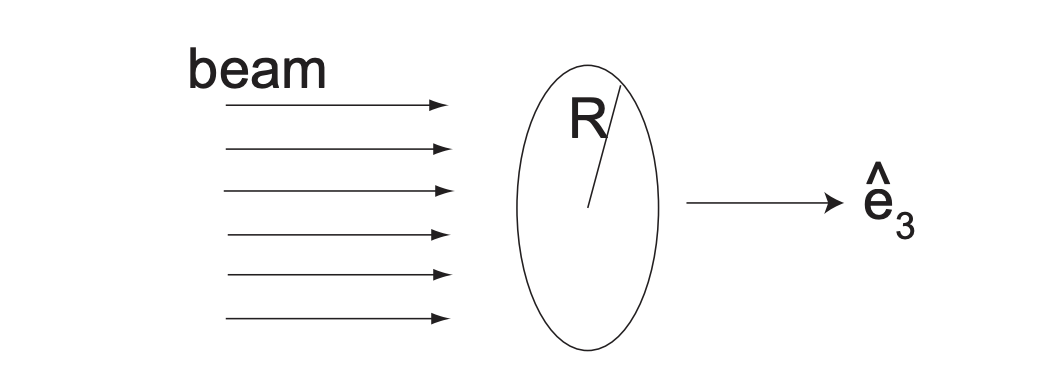
\includegraphics[width=0.5\textwidth]{gaussian.png}
\end{figure}

(c) For your generalized result of part (a), try to repeat our limiting case argument to obtain the "fundamental" cross section.
\section{}
\begin{enumerate}
  \setcounter{enumi}{31}
  \item We discussed the Ahronov-Bohm effect. Let us make some further interesting observations.
\end{enumerate}
\subsection{}
(a) Consider again the path integral in the vicinity of the long thin solenoid. In particular, consider a path which starts at $\boldsymbol{x}$, loops around the solenoid, and returns to $\boldsymbol{x}$. Since the $\boldsymbol{B}$ and $\boldsymbol{E}$ fields are zero everywhere in the region of the path, the only effect on the particle's wave function in traversing this path is a phase shift, and the amount of phase shift depends on the magnetic flux in the solenoid, as we discussed in class. Suppose we are interested in a particle with charge of magnitude $e$ (e.g., an electron). Show that the magnetic flux $\Phi$ in the solenoid must be quantized, and give the possible values that $\Phi$ can have.\\
In a previous problem said, we showed that when the particle completes a loop $C$ around that solenoid the wave function undergoes the transformation:
\begin{equation}
\psi \rightarrow e^{i q \oint_C \boldsymbol{A} \cdot d \boldsymbol{l}} \psi
\end{equation}
Stokes huron tells as that:
\begin{equation}
\oint_C \boldsymbol{A} \cdot d \boldsymbol{l} = \int_S \nabla \times \boldsymbol{A} \cdot d \boldsymbol{S}
\end{equation}
But from maxwell's equations we can simplify the integral on the right hand side:
\begin{equation}
\int_S \nabla \times \boldsymbol{A} \cdot d \boldsymbol{S} = \int_S \boldsymbol{B} \cdot d \boldsymbol{S}
\end{equation}
But we know that the magnetic killed is zero everywhere outside of the solenoid, so the only contribution to the integral on the red hand side is from the inside of the solenoid, which gives the magnetic flux through the solenoid:
\begin{equation}
\int_S \boldsymbol{B} \cdot d \boldsymbol{S} = \Phi
\end{equation}
Returning to our original expression, we know that the wave function at the start of the path has to equal the wave function at the end of the path, so the exponential factor has to be equal to unity:
\begin{equation}
e^{i q \Phi} = 1
\end{equation}
This brings about a condition for the magnetic flux:
\begin{equation}
q \Phi = 2 \pi n
\end{equation}
Where $n$ is an integer. This gives us the possible values for the magnetic flux:
\begin{equation}
\Phi = \frac{2 \pi n}{q}
\end{equation}
\subsection{}
(b) The BCS theory for superconductivity assumes that the basic "charge carrier" in a superconductor is a pair of electrons (a "Cooper pair"). The Meissner effect for a (Type I) superconductor is that when such a material is placed in a magnetic field, and then cooled below a critical temperature, the magnetic field is excluded from the superconductor. Suppose that there is a small nonsuperconducting region traversing the superconductor, in which magnetic flux may be "trapped" as the material is cooled below the critical temperature. What values do you expect to be possible for the trapped flux? [This effect has been experimentally observed.]\\
For the cooper pair, it will be a similar situation to that of the previous problem, but now we have a charge of $2q$ instead of $q$. So the possible values for the trapped flux will be:
\begin{equation}
\Phi = \frac{2 \pi n}{2q} = \frac{\pi n}{q} 
\end{equation}
\subsection{}
(c) So far, no one has observed (at least not convincingly) a magnetic "charge", analogous to the electric charge. But there is nothing fundamental that seems to prevent us from modifying Maxwell's equations to accommodate the existence of such a "magnetic monopole". In particular, we may alter the divergence equation to (in CGS gaussian units):

$$
\nabla \cdot \boldsymbol{B}=4 \pi \rho_{M},
$$

where $\rho_{M}$ is the magnetic charge density.

Consider a magnetic monopole of strength $e_{M}$ located at the origin. The $\boldsymbol{B}$-field due to this charge is simply:

$$
\boldsymbol{B}=\frac{e_{M}}{r^{2}} \hat{\boldsymbol{r}}
$$

where $\hat{\boldsymbol{r}}$ is a unit vector in the radial direction. The $\hat{\boldsymbol{r}}$-component of the curl of the vector potential is:

$$
\frac{1}{r \sin \theta} \frac{\partial}{\partial \theta}\left(A_{\phi} \sin \theta\right)-\frac{\partial A_{\theta}}{\partial \phi}
$$

A solution, as you should quickly convince yourself, is a vector potential in the $\phi$ direction:

$$
A_{\phi}=e_{M} \frac{1-\cos \theta}{r \sin \theta} .
$$

Unfortunately(?), this is singular at $\theta=\pi$, i.e., on the negative $z$-axis. We can fix this by using this form everywhere except in a cone about $\theta=\pi$, i.e., for $\theta \leq \pi-\epsilon$, and use the alternate solution:

$$
A_{\phi}^{\prime}=e_{M} \frac{-1-\cos \theta}{r \sin \theta}
$$

in the (overlapping) region $\theta \geq \epsilon$, thus covering the entire space. In the overlap region $(\epsilon \leq \theta \leq \pi-\epsilon)$, either $\boldsymbol{A}$ or $\boldsymbol{A}^{\prime}$ may be used, and must give the same result, i.e., the two solutions are related by a gauge transformation - that is, they differ by the gradient of a scalar function.

Consider the effect of the vector potential on the wave function of an electron (charge $-e$ ). Invoke single-valuedness of the wave function, and determine the possible values of $e_{M}$ that a magnetic charge can have. [This is sometimes called a "Dirac monopole".]\\
Within the domain of overlock of these two  solutions, they have to be equal up to a gauge transformation, so we can write:
\begin{equation}
A_{\phi} = A_{\phi}^{\prime} + \nabla \chi
\end{equation}
on the domain of overlap. We can write the difference between the two solutions as:
\begin{equation}
A_{\phi} - A_{\phi}^{\prime} = \nabla \chi
\end{equation} 
Substituting in for the left and side gives:
\begin{equation}
\frac{2e_M}{r\sin(\theta)} \hat{\phi } = \nabla \chi
\end{equation}
Then we know that the definition of the gradient and spherical coordinates is:
\begin{equation}
\nabla \chi = \hat{r} \frac{\partial \chi}{\partial r} + \hat{\theta} \frac{1}{r} \frac{\partial \chi}{\partial \theta} + \hat{\phi} \frac{1}{r \sin(\theta)} \frac{\partial \chi}{\partial \phi}
\end{equation}
By inspection we see that this has to be the third term because of the dependence on the united vector in the $\phi$ direction. So we can write:
\begin{equation}
\frac{2e_M}{r\sin(\theta)} = \frac{1}{r \sin(\theta)} \frac{\partial \chi}{\partial \phi}
\end{equation}
This implies that:
\begin{equation}
2e_M = \frac{\partial \chi}{\partial \phi} \rightarrow \chi = 2e_M \phi
\end{equation}
Now we go back to consider the relation between the initial and final wave function at the same point from the previous part of this question:
\begin{equation}
\psi \rightarrow e^{i q \oint_C \boldsymbol{A} \cdot d \boldsymbol{l}} \psi
\end{equation}
But now, this also has to hold under the gauge transformation:
\begin{equation}
\hat{A} \rightarrow \hat{A} + \nabla \chi
\end{equation}
So this gives a term that has to be invisible under the gauge transformation:
\begin{equation}
e^{i q \oint \nabla \chi \cdot d \boldsymbol{l}} = 1
\end{equation}
Now we know that the gradient of our scaler function is:
\begin{equation}
\nabla \chi = \nabla (2e_M \phi) = 2e_M \hat{\phi}
\end{equation}
If we take $\dd {\boldsymbol{l}} = \dd{\phi} \hat{\phi}$, then we can write:
\begin{equation}
\oint \nabla \chi \cdot d \boldsymbol{l} = \oint 2e_M \hat{\phi} \cdot \dd{\phi} \hat{\phi} = 2e_M \oint \dd{\phi} = 2e_M \Delta \phi
\end{equation}
Since we are choosing a path $\gamma $ that circles around the equator in our diagram, this line integral just evaluates to $2\pi$, so we can write:
\begin{equation}
\oint \nabla \chi \cdot d \boldsymbol{l} = 2e_M 2\pi = 4\pi e_M
\end{equation}
Since we need the condition for invisibility:
\begin{equation}
e^{i q \oint \nabla \chi \cdot d \boldsymbol{l}} = e^{i q 4\pi e_M} = 1 \rightarrow q 4\pi e_M = 2\pi n \rightarrow e_M = \frac{n}{2q}
\end{equation}
\begin{figure}
  \centering
  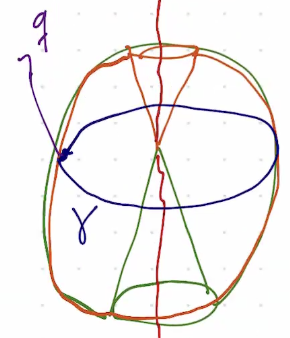
\includegraphics[width=0.5\textwidth]{dirac.png}
\end{figure}

\end{document}